\documentclass[12pt,a4paper]{uebung}

\usepackage[british]{babel}
\usepackage{epsfig}
\usepackage{rotate}
\usepackage{amsmath}
\usepackage{color}
\makeatletter\let\@amsfonts=P\makeatother
\usepackage{graphicx}
\usepackage{typearea}
\usepackage{multicol}
\usepackage{amsfonts}
\usepackage[nounderscore]{syntax}
\usepackage{paralist}
\usepackage{tikz}
\usepackage{url}
\usepackage{xspace}
\usepackage{listings}
\usepackage[ruled]{algorithm2e}
\def\NN{{\ensuremath{\mathbbm{N}_0\xspace}}}
\usepackage{fvsw}
\usepackage{tabularx}

\setlength{\textheight}{25cm}

\begin{document}

\newcommand{\Vorlesung}{Formal Methods in Computer Science}
\newcommand{\Semester}{SS 2012}
\newcommand{\Prof}{Univ.~Prof.~Helmut Veith}
\newcommand{\AssisA}{Dr. Igor Konnov}
\newcommand{\AssisB}{Dr. Florian Zuleger}
\newcommand{\AssisC}{Andreas Holzer, M.Sc.}
\newcommand{\AssisD}{Moritz Sinn, M.Sc.}

\newcommand{\solution}[1]{}

\newcommand\ltlX{\textsf{\textbf{X}}\,}
\newcommand\ltlF{\textsf{\textbf{F}}\,}
\newcommand\ltlG{\textsf{\textbf{G}}\,}
\newcommand\ltlU{\,\textsf{\textbf{U}}\,}
\newcommand\ILTLX[0]{$\mbox{\textsf{ILTL}}_{\mbox{\textsf{-X}}}$}
\newcommand\LTLX[0]{$\mbox{\textsf{LTL}}_{\mbox{\textsf{-X}}}$}

%%%%%%%%%%%%%%%%%%%%%%%%%%%%%%%%%%%%%%%%%%%%%%%%%%%%%%%%%%%%%%%%%%%%%%%%%%%%%%

\Uebungsblatt{4}{Wednesday, 30 May 2012}

%%%%%%%%%%%%%%%%%%%%%%%%%%%%%%%%%%%%%%%%%%%%%%%%%%%%%%%%%%%%%%%%%%%%%%%%%%%%%%

\setlength{\unitlength}{1mm}

\begin{tabularx}{\textwidth}{|l|X|}
\hline
\textbf{Name:}& Mustermann \\\hline
\textbf{Vorname:}& Max\\\hline
\textbf{Matr.-nr.:}& 0123456 \\\hline
\textbf{Gruppe:}& Neururer (0015595), Mayerhofer (0726179), Lang (0608292)  \\\hline
\end{tabularx}


%%%%%%%%%%%%%%%%%%%%%%%%%%%%%%%%%%%%%%%%%%%%%%%%%%%%%%%%%%%%%%%%%%%%%%
%% Aufgabe

\begin{center}
\textbf{The deadline for handing in the solution is Sunday, 17th of June, before midnight.}
\end{center}

\Aufgabe[ACTL \& LTL\hfill\textbf{(2 Points)}]
\newcommand{\ACTL}{\mathbf{ACTL}}
\newcommand{\LTL}{\mathbf{LTL}}
\newcommand{\CTLstar}{\mathbf{CTL}^*}
\newcommand{\AP}{\mathbf{AP}}
\newcommand{\true}{\mathbf{true}}
\newcommand{\false}{\mathbf{false}}
\newcommand{\trans}{\mathsf{trans}}
Given an LTL formula $\varphi$ in Negation Normal Form, the following function 
$\mathsf{trans} : \LTL \rightarrow \ACTL$ translates $\varphi$ into an ACTL 
formula $\trans(\varphi)$ as follows:
\begin{center}
\begin{tabular}{l|l}
	$\varphi$ & $\trans(\varphi)$\\
	\hline
	$\true$ & $\true$\\
	$\false$ & $\false$\\
	$a$ & $a$\\
	$\neg a$ & $\neg a$\\
	$\varphi_1 \vee \varphi_2$ & $\trans(\varphi_1) \vee \trans(\varphi_2)$\\
	$\varphi_1 \wedge \varphi_2$ & $\trans(\varphi_1) \wedge \trans(\varphi_1)$\\
	$\mathbf{X} \varphi_1$ & $\mathbf{AX}~\trans(\varphi_1)$\\
	$\mathbf{F} \varphi_1$ & $\mathbf{AF}~\trans(\varphi_1)$\\
	$\mathbf{G} \varphi_1$ & $\mathbf{AG}~\trans(\varphi_1)$\\
	$\varphi_1 \mathbf{U} \varphi_2$ & $\mathbf{A}\left[ \trans(\varphi_1)\;\mathbf{U}\;\trans(\varphi_2) \right]$\\
	$\varphi_1 \mathbf{R} \varphi_2$ & $\mathbf{A}\left[ \trans(\varphi_1)\;\mathbf{R}\;\trans(\varphi_2) \right]$\\
\end{tabular}
\end{center}
The semantics of the ``release'' operator $\mathbf{R}$ is defined as follows:
$$M, \pi \models \varphi_1 \mathbf{R} \varphi_2 \stackrel{def}{\Leftrightarrow} \forall j \geq 0. \pi^j \models \varphi_2 \textnormal{ or } \exists i \geq 0. (\pi^i \models \varphi_1) \wedge (\forall k \leq i. \pi^k \models \varphi_2)$$

\paragraph{a)} Show that, for all $\LTL$ formulas $\varphi$ in negation normal form, the $\CTLstar$ 
formula $\trans(\varphi) \Rightarrow \mathbf{A}\varphi$ is a tautology.
\emph{Hint: Show this by showing that $M, s \models \trans(\varphi)$ implies 
$M, s \models \mathbf{A}\varphi$ for all $\LTL$ formulas $\varphi$ in negation normal form, all Kripke 
structures $M$ and all states $s$ in $M$.
Use induction over the structure of~$\varphi$.}\hfill\textbf{(1 Point)}


\paragraph{b)} Show that, in general, $M, s \models \varphi$ does not imply $M, s \models \trans(\varphi)$.
\emph{Hint: Give a Kripke structure $M$ and an $\LTL$ formula $\varphi$ such that $M, s \models \varphi$ and $M, s \not\models \trans(\varphi)$. Discuss why $M, s \models \varphi$ and $M, s \not\models \trans(\varphi)$ holds on $M$ and the given state $s$ in $M$.}\\{\color{white} whitespace}\hfill\textbf{(1 Point)}




\newpage
\Aufgabe[LTL - Monotonicity and Negation Normal Form \hfill\textbf{(2 Point)}]

\begin{enumerate}

\item Let $K_1 = (S, R, L_1)$ and  $K_2 = (S, R, L_2)$ be two Kripke structures with the same set of states $S$ and the same transition relation $R$ such that $L_1(s) \subseteq L_2(s)$ for all states $s \in S$.
    Prove that $K_1,s \models \phi$ implies $K_2,s \models \phi$ for all LTL formulae $\phi$ that do not contain negation.
    \emph{(Hint: prove this statement by structural induction)}.

\item

Exercise 1 defined the \emph{release operator} \textbf{R}.
Prove that the release operator enjoys the following equivalence using the semantics of LTL \emph{(Hint: use the semantics of LTL formulae)}:
\begin{displaymath}
    \phi \mathbf{R} \psi \equiv \neg(\neg \psi \mathbf{U} \neg \phi)
\end{displaymath}

\item

An LTL formula in \emph{negation normal form}, if
\begin{itemize}
\item all negations appear only in front of the atomic propositions,
\item only the logical operators \emph{true}, \emph{false}, $\vee$, and $\wedge$ are used, and
\item only the temporal operators \textbf{X}, \textbf{U}, and \textbf{R} are used.
\end{itemize}

Show that every LTL formula $\phi$ can be transformed into an equivalent formula $\psi$ that is in negation normal form.
\emph{(Hint: prove this statement by structural induction)}.

\end{enumerate}

b.)
\textbf{Solution:}

\bigskip

The release-operator $\mathbf{R}$ is defined by%
\begin{equation}
\varphi \mathbf{R}\psi \equiv \lnot (\lnot \varphi \mathbf{U\lnot }\psi )
\label{release_op}
\end{equation}

and its interpretation is as follows. The formula $\varphi \mathbf{R}\psi $
holds if $\psi $ remains true, i.e. always holds, up to and including a
moment $i\geq 0$, when $\varphi $ becomes valid (if there is such a
(required) moment such that $\psi $ get released).

Let $2^{AP}$ be an alphabeth over $AP$. Then formally, the equivalence (\ref%
{release_op}) can be proven by using \ the semantics of the LTL\ formulae
over all Kripke structures $M$ and a given infinite word $%
s=a_{0}a_{1}a_{2}\ldots \in (2^{AP})^{w}$ such that:%

\renewcommand\thefootnote{\fnsymbol{footnote}}

\begin{eqnarray*}
M,s &\vDash &\lnot \psi  \\
&\Leftrightarrow &\text{\qquad (by def. of the operator }\mathbf{U}\text{
and the negation of it)} \\
\lnot \Exists j &\geq &0\,(M,s_{j}\vDash \lnot \psi \AND\Forall %
i<j.M,s_{i}\vDash \lnot \varphi ) \\
&\Leftrightarrow &\text{\qquad (by semantics of negation)} \\
\lnot \Exists j &\geq &0\,(M,s_{j}\nvDash \psi \AND\Forall %
i<j.M,s_{i}\nvDash \varphi ) \\
&\Leftrightarrow &\text{\qquad (by the duality of }\exists \text{ and }%
\forall \text{)} \\
\Forall j &\geq &0\,\lnot (M,s_{j}\nvDash \psi \AND\Forall %
i<j.M,s_{i}\nvDash \varphi ) \\
&\Leftrightarrow &\text{\qquad (using the law of de Morgan)} \\
\Forall j &\geq &0\,(\lnot (M,s_{j}\nvDash \psi )\OR\lnot \Forall %
i<j.M,s_{i}\nvDash \varphi ) \\
&\Leftrightarrow &\text{\qquad (by semantics of negation)} \\
\Forall j &\geq &0\,(M,s_{j}\vDash \psi \OR\underbrace{\Exists %
i<j.M,s_{i}\vDash \varphi}_{(\dag)})\;^{(}\footnotemark^{)} \\
&\Leftrightarrow &\text{\qquad (by (}\footnotemark\text{))} \\
\Forall j &\geq &0.\,M,s_{j}\vDash \psi \quad \text{or\quad }(\Exists i\geq
0.M,s_{i}\vDash \varphi \AND\Forall k\leq i.M,s_{k}\vDash \varphi ).
\end{eqnarray*}%

\addtocounter{footnote}{-1}
\footnotetext{%
This is equivalent to the common definition of $\mathbf{R}$, s. t. 
\begin{equation*}
M.\pi \vDash \varphi \mathbf{R}\psi \quad \text{iff}\quad \Forall j\geq 0%
\text{, then for every }i<j\text{, s.t. } \underbrace{M,\pi ^{i}\nvDash \varphi \IMPL %
M,\pi ^{j}\vDash \psi. }_{\lnot (M,\pi ^{i}\nvDash \varphi )\OR M,\pi
^{j}\vDash \psi }
\end{equation*}%
}
\stepcounter{footnote}
\footnotetext{Since $j\geq 0$ and $i$ cannot be $< 0$, i.e. $\Exists i\geq 0$, then
$\Forall j\geq 0$ and $\Exists i < j$ implies that $\Forall i \leq j$. To avoid confusion,
we have to introduce a new variable $k$ and substitution, s.t. $i\rightarrow k$ and $j\rightarrow i$.}

\newpage
\Aufgabe[Bisimulation \& Simulation Relations\hfill\textbf{(1 Point)}]

Consider the following Kripke structures $K_1$ and $K_2$ and the bisimulation relation $$H = \{ (s_0, t_0), (s_1, t_1), (s_2, t_2), (s_3, t_3), (s_4, t_4), (s_5, t_5), $$
$$(s_6, t_6), (s_6, t_7), (s_7, t_8), (s_8, t_9), (s_9, t_{10}) \}.$$

\begin{center}
\begin{minipage}{0.48\textwidth}
	\scalebox{0.8}{
  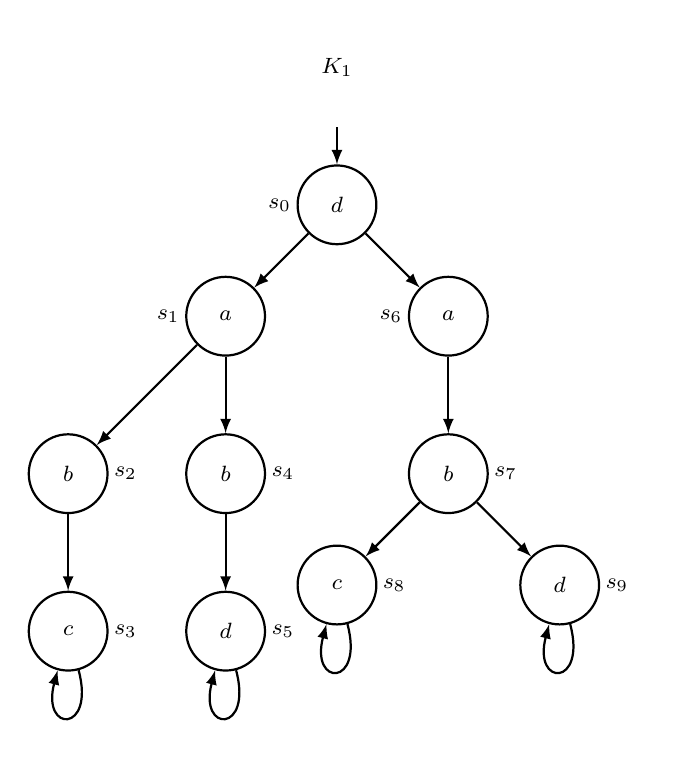
\begin{tikzpicture}[->,scale=1,label distance=-3mm,>= latex, node distance = 2cm]
    \tikzstyle{every node}=[shape=circle,minimum size=10mm,font=\footnotesize];
    \tikzstyle{every path} = [draw,thick];
    
    \node[draw] (n0) [label=left:$s_0$] {$d$};
    
    \node (tmp) [above of=n0, node distance=1.5cm] {};
    \node (tmp2) [above of=tmp,node distance=0.25cm] {$K_1$};
    
    \node[draw] (n6) [below right of=n0,label=left:$s_6$] {$a$};
    \node[draw] (n1) [below left of=n0,label=left:$s_1$] {$a$};
    \node[draw] (n4) [below of=n1,label=right:$s_4$] {$b$};
    \node[draw] (n2) [left of=n4,label=right:$s_2$] {$b$};
    \node[draw] (n3) [below of=n2,label=right:$s_3$] {$c$};
    \node[draw] (n5) [below of=n4,label=right:$s_5$] {$d$};
    \node[draw] (n8) [below of=n6,label=right:$s_7$] {$b$};
    \node[draw] (n9) [below left of=n8,label=right:$s_8$] {$c$};
    \node[draw] (n10) [below right of=n8,label=right:$s_{9}$] {$d$};
    
    \draw[->] (tmp) -- (n0);
    \draw[->] (n0) -- (n1);
    \draw[->] (n0) -- (n6);
    \draw[->] (n1) -- (n2);
    \draw[->] (n1) -- (n4);
    \draw[->] (n2) -- (n3);
    \draw[->] (n4) -- (n5);
		\draw[->] (n6) -- (n8);
		\draw[->] (n8) -- (n9);
		\draw[->] (n8) -- (n10);
		    
    \path[loop below] (n3) to (n3);
    \path[loop below] (n5) to (n5);
    \path[loop below] (n9) to (n9);
    \path[loop below] (n10) to (n10);
    
\end{tikzpicture}
}
\end{minipage}
\hfill
\begin{minipage}{0.48\textwidth}
	\scalebox{0.8}{
  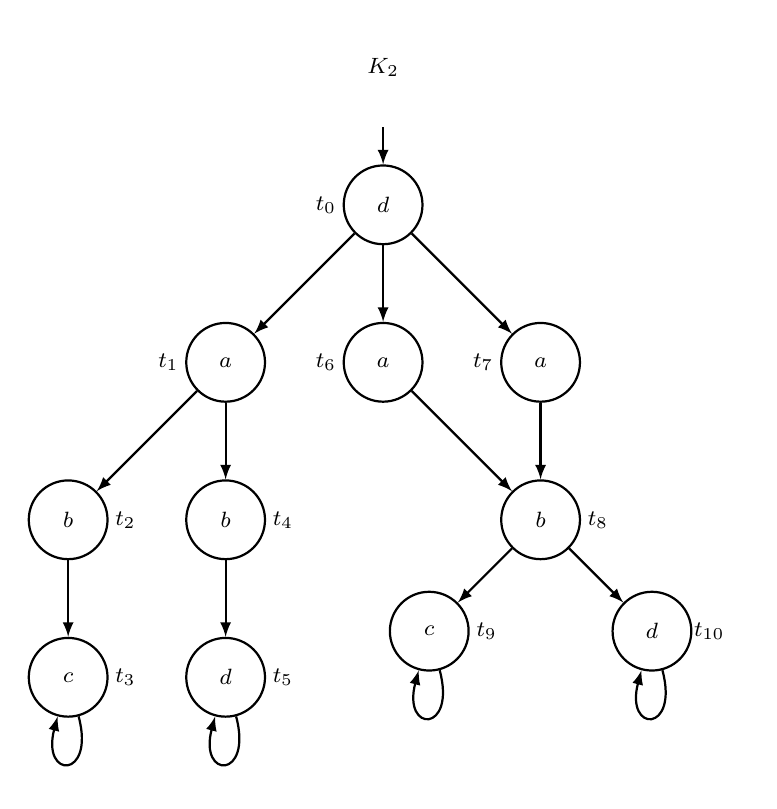
\begin{tikzpicture}[->,scale=1,label distance=-3mm,>= latex, node distance = 2cm]
    \tikzstyle{every node}=[shape=circle,minimum size=10mm,font=\footnotesize];
    \tikzstyle{every path} = [draw,thick];
    
    \node[draw] (n0) [label=left:$t_0$] {$d$};
    
    \node (tmp) [above of=n0, node distance=1.5cm] {};
    \node (tmp2) [above of=tmp,node distance=0.25cm] {$K_2$};
    
    \node[draw] (n6) [below of=n0,label=left:$t_6$] {$a$};
    \node[draw] (n1) [left of=n6,label=left:$t_1$] {$a$};
    \node[draw] (n7) [right of=n6,label=left:$t_7$] {$a$};
    \node[draw] (n4) [below of=n1,label=right:$t_4$] {$b$};
    \node[draw] (n2) [left of=n4,label=right:$t_2$] {$b$};
    \node[draw] (n3) [below of=n2,label=right:$t_3$] {$c$};
    \node[draw] (n5) [below of=n4,label=right:$t_5$] {$d$};
    \node[draw] (n8) [below of=n7,label=right:$t_8$] {$b$};
    \node[draw] (n9) [below left of=n8,label=right:$t_9$] {$c$};
    \node[draw] (n10) [below right of=n8,label=right:$t_{10}$] {$d$};
    
    \draw[->] (tmp) -- (n0);
    \draw[->] (n0) -- (n1);
    \draw[->] (n0) -- (n6);
    \draw[->] (n0) -- (n7);
    \draw[->] (n1) -- (n2);
    \draw[->] (n1) -- (n4);
    \draw[->] (n2) -- (n3);
    \draw[->] (n4) -- (n5);
		\draw[->] (n6) -- (n8);
		\draw[->] (n7) -- (n8);
		\draw[->] (n8) -- (n9);
		\draw[->] (n8) -- (n10);
		    
    \path[loop below] (n3) to (n3);
    \path[loop below] (n5) to (n5);
    \path[loop below] (n9) to (n9);
    \path[loop below] (n10) to (n10);
    
\end{tikzpicture}
}
\end{minipage}
\end{center}


\paragraph{a)} Give a simulation relation $H'$ such that $K_1 \leq K_2$ and $|H'| < |H|$.\hfill\textbf{(0.5 Points)}
\\

$\ddot\smile$ \textbf{Solution}\\
To get the wanted simulation relation $H'$ you can remove either $(s_6,s_6)$ or $(s_6,s_7)$ from $H$.\\
We removed $(s_6,s_6)$ and got
$$H' = \{ (s_0, t_0), (s_1, t_1), (s_2, t_2), (s_3, t_3), (s_4, t_4), (s_5, t_5), $$
$$(s_6, t_7), (s_7, t_8), (s_8, t_9), (s_9, t_{10}) \}.$$

$|H'| = 10 < |H| = 11 \checkmark$

\paragraph{b)} Give a simulation relation $H''$ such that $K_1 \leq K_2$ and $|H''| > |H|$.\hfill\textbf{(0.5 Points)}
\\

$\ddot\smile$ \textbf{Solution}\\
There are a lot of possibilities, we've chosen this:\\
$$H'' = \{ (s_0, t_0), (s_1, t_1), (s_2, t_2), (s_3, t_3), (s_4, t_4), (s_5, t_5), $$
$$(s_6, t_6), (s_6, t_7), (s_7, t_8), (s_8, t_9), (s_9, t_{10}), (s_2,t_8), (s_4, t_8) \}.$$

$|H''| = 13 > |H| = 11 \checkmark$

\newpage
\Aufgabe[Simulation as refinement \hfill\textbf{(2 Points)}]
 
Given a \texttt{C} program and a set $AP$ of atomic propositions,
one can construct a Kripke structure over $AP$ which models the behaviour of the program with respect to the atomic propositions. 
For example, given the following program:

\begin{verbatim}
int x = 0, y = 0;
l0:
    for (int i = 0; i < 2; i++)
l1:     x = 1;
    y = *;
    if (y != 0)
l2:     x = 1;
    else
l3:     x = 0;
    goto l0;
\end{verbatim}

One may construct the following Kripke structure over $AP=\{x=0, y=0\}$
as follows:

\begin{center}
	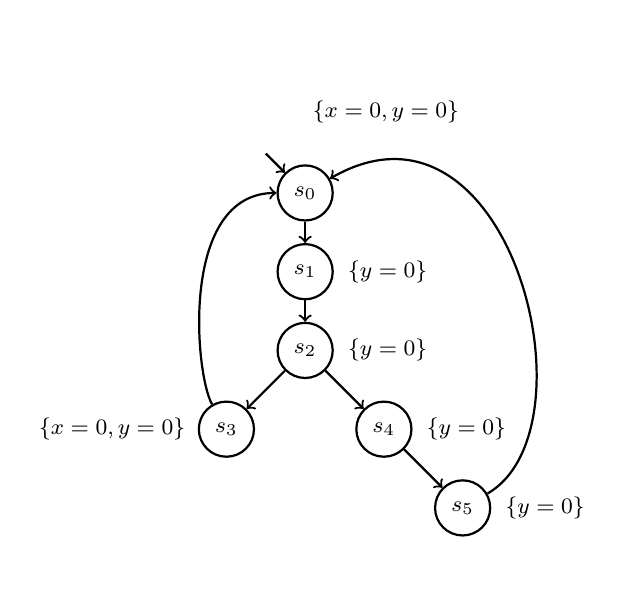
\begin{tikzpicture}[->,scale=1,label distance=0mm]
		\tikzstyle{every node}=[draw,shape=circle,minimum size=7mm,font=\footnotesize];
    \tikzstyle{every path}=[draw,thick];
    \node at (0, 0)   (s0) [label=above right:${ \{x=0,y=0\} }$]  {$s_0$};
    \node at (0, -1)  (s1) [label=right:${ \{y=0\} }$] {$s_1$};
    \node at (0, -2)  (s2) [label=right:${ \{y=0\} }$] {$s_2$};
    \node at (-1, -3) (s3) [label=left:${ \{x=0,y=0\} }$] {$s_3$};
    \node at (1, -3)  (s4) [label=right:${ \{y=0\} }$] {$s_4$};
    \node at (2, -4)  (s5) [label=right:${ \{y=0\} }$] {$s_5$};

    \draw (-0.5, 0.5) to (s0);
    \draw (s0) to (s1);
    \draw (s1) to (s2);
    \draw (s2) to (s3);
    \draw (s2) to (s4);
    \draw (s3) .. controls +(120:8mm) and +(left:16mm) .. (s0);
    \draw (s4) to (s5);
    \draw (s5) .. controls +(30:20mm) and +(30:30mm) .. (s0);
	\end{tikzpicture}
\end{center}
In the example above, the special
form of assignment \texttt{y = *} denotes a non-deterministic assignment
to~\texttt{y} of any value from the domain of \texttt{y}, e.g., it can be
assigned concurrently by another thread.
The effect of a statement sequence residing under the same label $\ell_j$ may
be merged into one state, whereas the effect of statements marked with
distinct labels $\ell_j$ and $\ell_k$, $j \ne k$, must not be merged into one
state.

\paragraph{a)}
Construct a Kripke structure $K$ over
$AP=\{port\_o=0,port\_o=1,port\_o=2,port\_o=3\}$ for the following program:

\begin{verbatim}
int locked_dev = 0, port_o = 0, port_i = 0;
l0:
    for (int i = 0; i < 3; i++)
l1:     port_o = 1;

    port_i = *;
    if (port_i < 3) {
        goto l0;
    }
    do {
l2:     port_o = 2; locked_dev = *;
    } while (locked_dev);
l3: locked_dev = 1; port_i = *;
    if (port_i == 1)
l4:     port_o = 1;
    else
l5:     port_o = 3;
l6: port_o = 0; locked_dev = 0;
    goto l0;
\end{verbatim}


\paragraph{b)}
Give simulation relations between $K$ and the following Kripke structures
 $S'$ (left) and $S''$ (right):

\begin{center}
	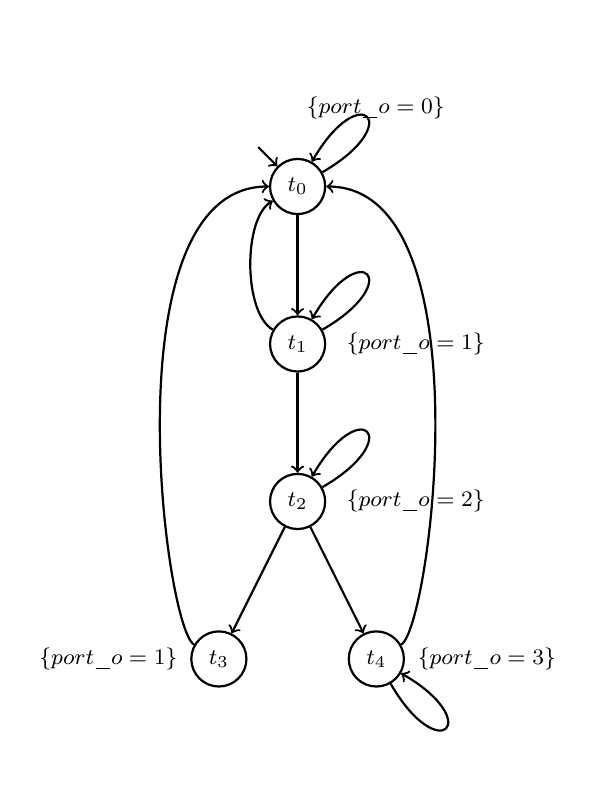
\begin{tikzpicture}[->,scale=1,label distance=0mm]
		\tikzstyle{every node}=[draw,shape=circle,minimum size=7mm,font=\footnotesize];
    \tikzstyle{every path}=[draw,thick];
    \node at (0, 0)   (s0) [label=above right:${ \{port\_o=0\} }$]  {$t_0$};
    \node at (0, -2)  (s1) [label=right:${ \ \{port\_o=1\} }$] {$t_1$};
    \node at (0, -4)  (s2) [label=right:${ \ \{port\_o=2\} }$] {$t_2$};
    \node at (-1, -6) (s3) [label=left:${ \{port\_o=1\} }$] {$t_3$};
    \node at (1, -6)  (s4) [label=right:${ \{port\_o=3\} }$] {$t_4$};

    \draw (-0.5, 0.5) to (s0);
    \draw (s0) to (s1);
    \draw (s0)  .. controls +(30:16mm) and +(60:16mm) .. (s0);
    \draw (s1)  .. controls +(150:8mm) and +(210:8mm) .. (s0);
    \draw (s1)  .. controls +(30:16mm) and +(60:16mm) .. (s1);
    \draw (s1) to (s2);
    \draw (s2)  .. controls +(30:16mm) and +(60:16mm) .. (s2);
    \draw (s2) to (s3);
    \draw (s2) to (s4);
    \draw (s3) .. controls +(150:8mm) and +(left:24mm) .. (s0);
    \draw (s4) .. controls +(30:8mm) and +(right:24mm) .. (s0);
    \draw (s4)  .. controls +(300:16mm) and +(330:16mm) .. (s4);
    	\end{tikzpicture}
	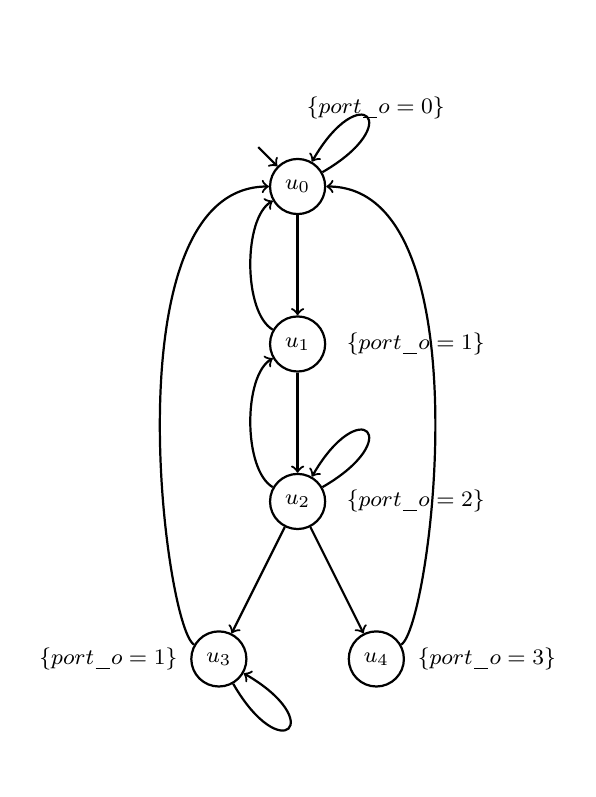
\begin{tikzpicture}[->,scale=1,label distance=0mm]
		\tikzstyle{every node}=[draw,shape=circle,minimum size=7mm,font=\footnotesize];
    \tikzstyle{every path}=[draw,thick];
    \node at (0, 0)   (s0) [label=above right:${ \{port\_o=0\} }$]  {$u_0$};
    \node at (0, -2)  (s1) [label=right:${ \ \{port\_o=1\} }$] {$u_1$};
    \node at (0, -4)  (s2) [label=right:${ \ \{port\_o=2\} }$] {$u_2$};
    \node at (-1, -6) (s3) [label=left:${ \{port\_o=1\} }$] {$u_3$};
    \node at (1, -6)  (s4) [label=right:${ \{port\_o=3\} }$] {$u_4$};

    \draw (-0.5, 0.5) to (s0);
    \draw (s0) to (s1);
    \draw (s0)  .. controls +(30:16mm) and +(60:16mm) .. (s0);
    \draw (s1)  .. controls +(150:8mm) and +(210:8mm) .. (s0);
    \draw (s2)  .. controls +(150:8mm) and +(210:8mm) .. (s1);
    \draw (s1) to (s2);
    \draw (s2)  .. controls +(30:16mm) and +(60:16mm) .. (s2);
    \draw (s2) to (s3);
    \draw (s2) to (s4);
    \draw (s3) .. controls +(150:8mm) and +(left:24mm) .. (s0);
    \draw (s3) .. controls +(300:16mm) and +(330:16mm) .. (s3);
    \draw (s4) .. controls +(30:8mm) and +(right:24mm) .. (s0);
    	\end{tikzpicture}
\end{center}

$\ddot\smile$ \textbf{Solution}\\
\begin{enumerate}
\item
Kripke structure $K$:
\begin{center}
	\begin{tikzpicture}[->,scale=1,label distance=0mm]
		\tikzstyle{every node}=[draw,shape=circle,minimum size=7mm,font=\footnotesize];
    \tikzstyle{every path}=[draw,thick];
    \node at (0, 0)   (s0) [label=right:${ \{port\_o=0\} }$]  {$s_0$};
    \node at (0, -2)  (s1) [label=upper right:${ \ \{port\_o=1\} }$] {$s_1$};
    \node at (0, -4)  (s2) [label=right:${ \ \{port\_o=1\} }$] {$s_2$};
    \node at (0, -6)  (s3) [label=bottom right:${ \ \{port\_o=1\} }$] {$s_3$};
    \node at (-1, -8) (s4) [label=left:${ \{port\_o=1\} }$] {$s_4$};
    \node at (1, -8)  (s5) [label=right:${ \{port\_o=2\} }$] {$s_5$};
    \node at (0, -10) (s6) [label=left:${ \{port\_o=1\} }$] {$s_6$};
    \node at (2, -10)  (s7) [label=right:${ \{port\_o=3\} }$] {$s_7$};
    \node at (1, -12)  (s8) [label=upper:${ \ \{port\_o=0\} }$] {$s_8$};

    \draw (-0.5, 0.5) to (s0);
    \draw (s0) to (s1);
    \draw (s1) to (s2);
    \draw (s2) to (s3);
    \draw (s3) to (s4);
    \draw (s3) to (s5);
    \draw (s4) .. controls +(150:8mm) and +(left:24mm) .. (s1);
    \draw (s5) .. controls +(30:16mm) and +(60:16mm) .. (s5);
    \draw (s5) to (s6);
    \draw (s5) to (s7);
    \draw (s6) to (s8);
    \draw (s7) to (s8);
    \draw (s8)  .. controls +(20:170mm) and +(20:60mm) .. (s0);
    	\end{tikzpicture}
\end{center}

\item
$S'$ simulates $K$ with the following simulation relation\\
$$H' = \{(s_0,t_0),(s_1,t_1),(s_2,t_1),(s_3,t_1),(s_4,t_1),(s_5,t_2),(s_6,t_3),(s_7,t_4),(s_8,t_0)\}.$$
ans $S''$ simulates $K$ with the following simulation relation\\
$$H'' = \{(s_0,u_0),(s_1,u_3),(s_2,u_3),(s_3,u_1),(s_4,u_3),(s_5,u_2),(s_6,u_3),(s_7,u_4),(s_8,u_0)\}.$$
$K$ doesn't simulate neither $S'$ nor $S''$, because there doesn't exist any state with AP $\{port\_o=0\}$ which has a path to $\{port\_o=0\}$ and $\{port\_o=1\}$...
\end{enumerate}

\newpage
\Aufgabe[Predicate Abstraction\hfill\textbf{(1.5 Point)}]
Consider the following program:
\begin{verbatim}
void foo(int j, int z) {
  assume(z != 0);
  int i := j;
  while(z != 0) {
      i := i + z;
      if(z > 0)
          z--
      else
          z ++;
  };
  assert(i != j)
}
\end{verbatim}

The {\em assume statement} at the beginning of the function forces the parameter $z$ not to be 0 when the function is called.

\begin{enumerate}

 \item Argue in your own words why the assertion at the end of the program allways holds, i.e., why the error state can never be reached.

 \item Provide a labeled transition system for the given program.

 \item Provide an abstraction for the labeled transition system that uses the predicates $i = j$, $i < j$, $i > j$.

 \item Check whether the error state can be reached in the abstraction, if so state a trace to the error state and refine the abstraction with suitable predicates such that the error state is not reachable anymore.

\end{enumerate}


\textbf{Solution:}\\
\medskip
\begin{enumerate}
\item The call of the method \texttt{\small assume(z != 0)} in the beginning
of the program forces, that the value of the variable $z$ is not $0$. Since
the semantics of \texttt{\small assume(x)}, means that "by assumption \texttt%
{\small x} holds" and by definition an assumption can never being violated.
Thus, the while-loop will be executed at least one time, regardless if the
value of $z$ is positive or negative.

Since the if-condition inside of the loop controls $z$ by decrementing or
incrementing and consequently the variable $i$ will also incremented or
decremented. Thus, the loop will be executed exactly in $|z|$ times. Since  $%
i=j$ is in the precondition of the loop, the loop is guaranteed to terminate
since $z\neq 0$. Hence, after the termination of the while-loop, the case
that $i=j$ will never reached, i.e. it will never hold.

\item
\newpage
\textit{Labeled Transiton System (LTS):}
\begin{figure}[th]
\centering
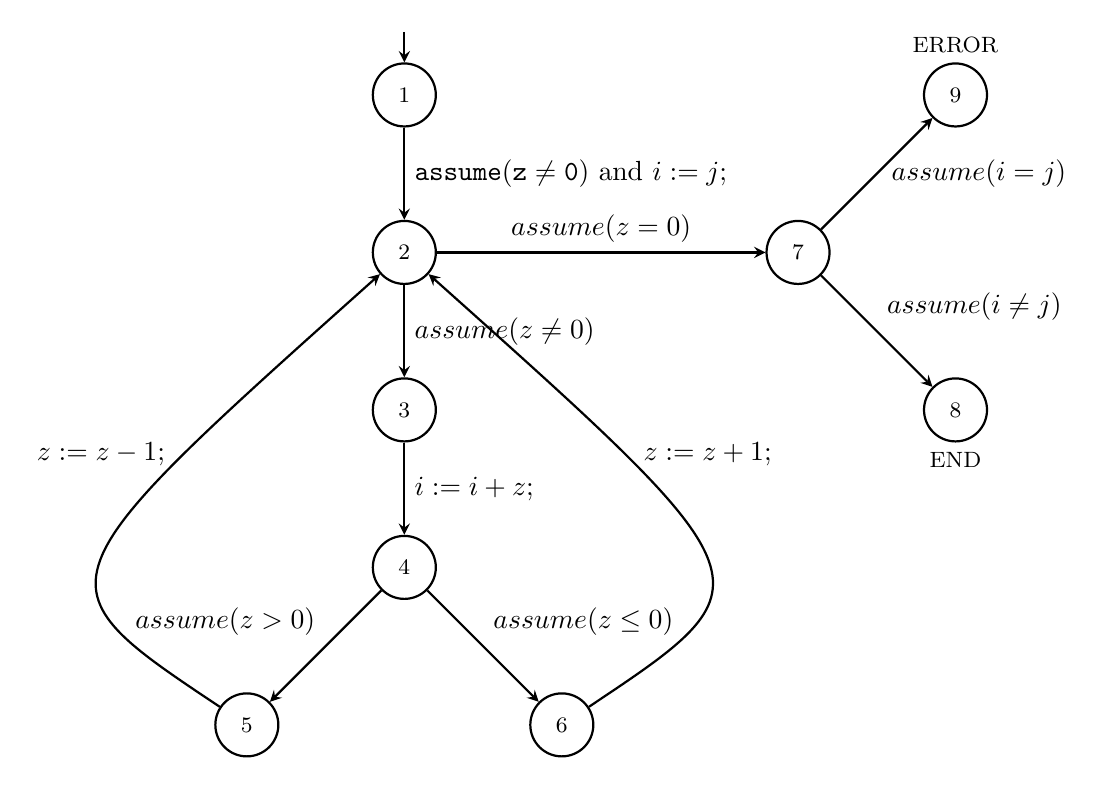
\begin{tikzpicture}[->, >=stealth, line join=bevel]
	\pgfsetlinewidth{1bp}
	\pgfsetcolor{black}

	\tikzstyle{state} = [draw,shape=circle,minimum size=8mm,font=\footnotesize];
	\tikzstyle{accept_state} = [shape=circle, minimum size=8mm, accepting, font=\small, draw];
	\tikzstyle{every path} = [draw, thick];

	\node[state] at (0,10) (1) {$1$};
	\node[state] at (0,8) (2) {$2$}; 
	\node[state] at (0,6) (3) {$3$}; 
	\node[state] at (0,4) (4) {$4$}; 
	\node[state] at (-2,2) (5) {$5$}; 
	\node[state] at (2,2) (6) {$6$}; 
	\node[state] at (5,8) (7) {$7$}; 
	\node[state] at (7,6) (8) [label=below:{\footnotesize END}] {$8$}; 
	\node[state] at (7,10) (9) [label=above:{\footnotesize ERROR}] {$9$}; 

	\draw (0, 10.8) to (1);
	\draw (1) to node[auto] {$\mbox{\fontsize{10}{11}\selectfont $\mathtt{assume(z \neq 0)} \mbox{ and } i := j;$}$} (2);
	\draw (2) to node[auto] {$\mbox{\fontsize{10}{11}\selectfont $assume(z \neq 0)$}$} (3);
	\draw (3) to node[auto] {$\mbox{\fontsize{10}{11}\selectfont $i := i+z;$}$} (4);
	\draw (4) to node[auto, swap] {$\mbox{\fontsize{10}{11}\selectfont $assume(z > 0)$}$} (5);
	\draw (4) to node[auto] {$\mbox{\fontsize{10}{11}\selectfont $assume(z \leq 0)$}$} (6);
	\draw (2) to node[auto] {$\mbox{\fontsize{10}{11}\selectfont $assume(z = 0)$}$} (7);
	\draw (7) to node[auto] {$\mbox{\fontsize{10}{11}\selectfont $assume(i \neq j)$}$} (8);
	\draw (7) to node[right] {$\mbox{\fontsize{10}{11}\selectfont $\,assume(i = j)$}$} (9);
	\draw[->] (5) .. controls (-4.7,3.8) .. (2) node[pos=.75, left] {$z := z-1;\;$};
	\draw[->] (6) .. controls (4.7,3.8) .. (2) node[pos=.75, right] {$\;z := z+1;$};
\end{tikzpicture}
\caption{{\protect\small LTS of the given program.}}
\label{lts_program}
\end{figure}

\item

Notation + Graph folgen noch

\item
There is no reachable error trace in the abstraction.
\end{enumerate}
\newpage
%%%%%%%%%%%%%%%%%%%%%%%%%%%%%%%%%%%%%%%%%%%%%%%%%%%%%%%%%%%%%%%%%%%%%%
%% Aufgabe
\Aufgabe[Bounded Model Checking\hfill\textbf{(1.5 Point)}]
Consider the following Program:

\lstinputlisting[basicstyle=\footnotesize]{main.c}

The Matrix $G$ models a graph with $N$ nodes, i.e, $G[i][j]$ is true iff there is a directed edge from node $i$ to node $j$. The method $\mathit{nondet}$ chooses an integer non-deterministically.

\begin{enumerate}
	\item Use CBMC to find the lowest value for $K$ such that the assertion at the end of the program can be violated. What does it mean that the error state is or is not reachable for a given graph $G$ and a given value $K$?

	\item Perform an unwinding of the loop for $K = 3$.
				
	\item Transform the unwinded program into the SSA form.
	
	\item Build a semantically equivalent SMT formula from the SSA form. {\em Note:} A call to $\mathit{nondet}$ can be modeled by introducing a new integer variable.

        \item Can you draw a conclusion about the satisfiability of the formula by comparing the value for $K$ that you determined under $(a)$ with the number of times the loop was unwinded for building the formula? Check whether the formula can be satisfied (You may use an SMT solver such as {\em Yices} or {\em Z3}) to be sure that the result of the satisfiability check is consistent with your expectation.

\end{enumerate}

\vspace{0.5cm}

$\ddot\smile$ \textbf{Solution}\\
\begin{enumerate}
\item
The lowest value $K$ for a violated assertion is $1$.

\item[(b) \& (c)] \quad
\medskip
\begin{lstlisting}[	frame=lines, mathescape=true,
					caption={ Unwinded code in SSA form:},
					label={unw_func}]
void main() {
	// Intialization:
	bool G[N][N] = {{$\ldots$}};
	bool result$_0$ = 1;
	int node$_0$ = 0;
	int next$_0$ = 0;
	int i$_0$ = 0;
	
	// Unwinding of the for-loop for $K = 3$:
	// First iteration:
	if(i$_0$ < K) {
		next$_1$ = nondet() % N;
		result$_1$ = result$_0$ && G[node$_0$][next$_1$];
		node$_1$ = next$_1$;
		i$_1$ = i$_0$ + 1;
		// Second iteration:
		if(i$_1$ < K) {
			next$_2$ = nondet() % N;
			result$_2$ = result$_1$ && G[node$_1$][next$_2$];
			node$_2$ = next$_2$;
			i$_2$ = i$_1$ + 1;
			result$_3$ = result$_2$;
			// Third iteration + termination:
			if(i$_2$ < K) {
				next$_3$ = nondet() % N;
				result$_3$ = result$_2$ && G[node$_2$][next$_3$];
				node$_3$ = next$_3$;
				i$_3$ = i$_2$ + 1;
				assert(!(i$_3$ < K));
			}
		}
	}
	result$_4$ = result$_3$ && node$_3$ == 0) && (K > 0);

	assert(!result$_4$);
}
\end{lstlisting}

\item[(d)]
\item[(e)]
\end{enumerate}
\newpage
\Aufgabe[Computing the (Greatest) Bisimulation Relation \hfill\textbf{(1 Point)}]

Let $K_1 = (S_1, R_1, L_1)$ and  $K_2 = (S_2, R_2, L_2)$ be two Kripke structures over a set of atomic predicates $\mathit{AP}$.
The relations $H_n \subseteq S_1 \times S_2$ are inductively defined by:
\begin{itemize}
\item $(s_1,s_2) \in H_0$ iff $L_1(s_1) = L_2(s_2)$.
\item $(s_1,s_2) \in H_{n+1}$ iff
    \begin{enumerate}[(i)]
    \item $(s_1,s_2) \in H_n$,
    \item for all $(s_1,t_1) \in R_1$ there exists a $(s_2,t_2) \in R_2$ with $(t_1,t_2) \in H_n$, and
    \item for all $(s_2,t_2) \in R_2$ there exists a $(s_1,t_1) \in R_1$ with $(t_1,t_2) \in H_n$.
    \end{enumerate}
\end{itemize}

\begin{enumerate}

	\item Compute the sequence $H_0, H_1, H_2,\ldots$ for the Kripke structures $K_1$ and $K_2$ from Exercise 2.
    
	\item Show that the sequence $H_0, H_1, H_2,\ldots$ \emph{stabilizes} for all finite Kripke structures $K_1$ and $K_2$, i.e., there is a $n \ge 0$ such that $H_n = H_{n+1}$.
    
	\item Construct Kripke structures $K_1^n$ and $K_2^n$ such that the sequence $H_0, H_1, H_2,\ldots$ stabilizes after exactly $n$ steps.

\end{enumerate}

\newpage

\end{document}

